\section{Theoretical Analysis}
\label{sec:analysis}

\paragraph{} The values used in both analysis are the following:


\begin{table}[h]
  \centering
  \begin{tabular}{|l|r|}
    \hline
    {\bf Name} & {\bf Value} \\ \hline
    $R_1$ & 1.001963 $k\Omega$\\ \hline
$R_2$ & 2.082319 $k\Omega$\\ \hline
$R_3$ & 3.057981 $k\Omega$\\ \hline
$R_4$ & 4.104964 $k\Omega$\\ \hline
$R_5$ & 3.036581 $k\Omega$\\ \hline
$R_6$ & 2.003567 $k\Omega$\\ \hline
$R_7$ & 1.049520 $k\Omega$\\ \hline
$V_S$ & 5.064003 $V$\\ \hline
$C$n& 1.019607 $uF$\\ \hline
$K_b$ & 7.026045 $mS$\\ \hline
$K_d$ & 8.359170 $mS$\\ \hline

  \end{tabular}
  \caption{Circuit data generated by inputing 86639 to the $t2\_datagen.py$ file.}                                                            
  \label{tab:data}                                                      
\end{table}   

\subsection{Analysis for t<0}

\paragraph{} For t<0 we can see that we are working in the steady state, given that in that time interval $v_S$ = $V_S$. In a DC circuit, the capacitor charges up to it's full capacity, blocking the flow of electricity. Taking 
this into account we can replace the capacitor with an open circuit. With this information, and knowing that the the tension in $V_4$, since it is connected to ground, we can obtain the following equations.

\begin{equation}
\begin{bmatrix}
	-1	&	0	&	0	&	0	&	0	&	0	&	0 \\
	G_1	&	-G_1 - G_2 - G_3	&	G_2	&	G_3	&	0	&	0	&	0 \\
	0	&	-K_b - G_2	&	G_2	&	K_b	&	0	&	0	&	0 \\
	G_1	&	-G_1	&	0	&	-G_4	&	0	&	-G_6	&	0 \\
	0	&	0	&	0	&	0	&	0	&	G_6 + G_7	&	-G_7 \\
	0	&	0	&	0	&	-1	&	0	&	-G_6 *	K_d	&	1 \\
	0	&	G_3	&	0	&	-G_3 - G_4 - G_5	&	G_5	&	-G_6	&	0
\end{bmatrix}
\times
\begin{bmatrix}
	V_1 \\
	V_2 \\
	V_3 \\
	V_5 \\
	V_6 \\
	V_7 \\
	V_8
\end{bmatrix}
=
\begin{bmatrix}
	-V_s \\
	0 \\
	0 \\
	0 \\
	0 \\
	0 \\
	0
	\label{m:1}
\end{bmatrix}
\end{equation}

After solving them with the Octave sofware, we obtained the following results:

\clearpage

\begin{table}[h]
  \centering
  \begin{tabular}{|l|r|}
    \hline
    {\bf Name} & {\bf Value} \\ \hline
    $V1$ & 5.048640 $V$\\ \hline
$V2$ & 4.860629 $V$\\ \hline
$V3$ & 4.468710 $V$\\ \hline
$V5$ & 4.888344 $V$\\ \hline
$V6$ & 5.496080 $V$\\ \hline
$V7$ & -2.026270 $V$\\ \hline
V8 & -3.015705 $V$\\ \hline
$I(R_1)$ & 0.186554 $mA$\\ \hline
$I(R_2)$ & 0.195655 $mA$\\ \hline
$I(R_3)$ & 0.009102 $mA$\\ \hline
$I(R_4)$ & 1.169750 $mA$\\ \hline
$I(R_5)$ & 0.195655 $mA$\\ \hline
$I(R_6)$ & 0.983196 $mA$\\ \hline
$I(R_7)$ & 0.983196 $mA$\\ \hline
$I(V_s)$ & 0.186554 $mA$\\ \hline
$I_b$ & -0.195655 $mA$\\ \hline
$I_c$ & 0.000000 $mA$\\ \hline
$I(K_d)$ & 0.983196 $mA$\\ \hline

  \end{tabular}
  \caption{Nodal Analysis for $t<0~s$. Currents are expressed in milliAmpere and Voltages are expressed in Volt.}                                                            
  \label{tab:theoretical1}                                                      
\end{table}   



\subsection{Equivalent Resistance and Initial Conditions}


\paragraph{}In order to determine the equivalent resistance we need to determine $V_X$, this is, the difference between $V_6$ - $V_8$. This is made to ensure that the voltage in the capacitor is continuous.

Making use of the matrix below:

\begin{equation}
\begin{pmatrix}
-1 & 0 & 0 & 0 & 0 & 0 & 0\\
G1 & -G1-G2-G3 & G2 & G3 & 0 & 0 & 0\\
0 & -Kb-G2 & G2 & Kb & 0 & 0 & 0\\
G1 & -G1 & 0 & -G4 & 0 & -G6 & 0\\
0 & 0 & 0 & 0 & 0 & G6+G7 & -G7\\
0 & 0 & 0 & -1 & 0 & -G6*Kd & 1\\
0 & 0 & 0 & 0 & -1 & 0 & 1\\
\end{pmatrix}
\begin{pmatrix}
V1\\
V2\\
V3\\
V5\\
V6\\
V7\\
V8\\
\end{pmatrix}
=
\begin{pmatrix}
0\\
0\\
0\\
0\\
0\\
0\\
-Vx\\
\end{pmatrix}
\end{equation}
\newpage
And knowing that:

\begin{equation}
	V_x = V_6 - V_8
\end{equation}

\begin{equation}
	I_x = \frac{V_6 - V_5}{R_5} + \frac{V_3 - V_2}{R_2}
\end{equation}

\begin{equation}
	R_eq = \frac{V_x}{I_x}
\end{equation}

\begin{equation}
	\tau = R_eq * C
\end{equation}

We can obtain the following values:

\begin{table}[h]
  \centering
  \begin{tabular}{|l|r|}
    \hline    
    {\bf Name} & {\bf Value} \\ \hline
    $V_x$ & 8.511786 $V$\\ \hline
$I_x$ & 2.740295 $mA$\\ \hline
$R_{Eq}$ & 3.106157 $k\Omega$\\ \hline
$\tau$ & 0.003184 $s$\\ \hline 
  \end{tabular}
  \caption{Second nodal analysis and calculations for $R_{Eq}$ and $\tau$. Currents are expressed in $milliAmpere$, Voltages are expressed in $Volt$, Resistances are expressed in $kiloOhm$ and Time Constant is expressed in $second$.}
  \label{tab:theoretical2}
\end{table}

\subsection{Natural Solution}


\paragraph{} The natural solution doesn't take into account independent power sources. Using $V_x$ as the initial condition the natural solution can be obtained with the following equation

\begin{equation}
	V_{6n}(t) = V_x e^{(-\frac{t}{\tau})}
\end{equation}

After computing this data on Octave, we can plot the results of the interval [0, 20]ms.


\begin{figure}[h] \centering
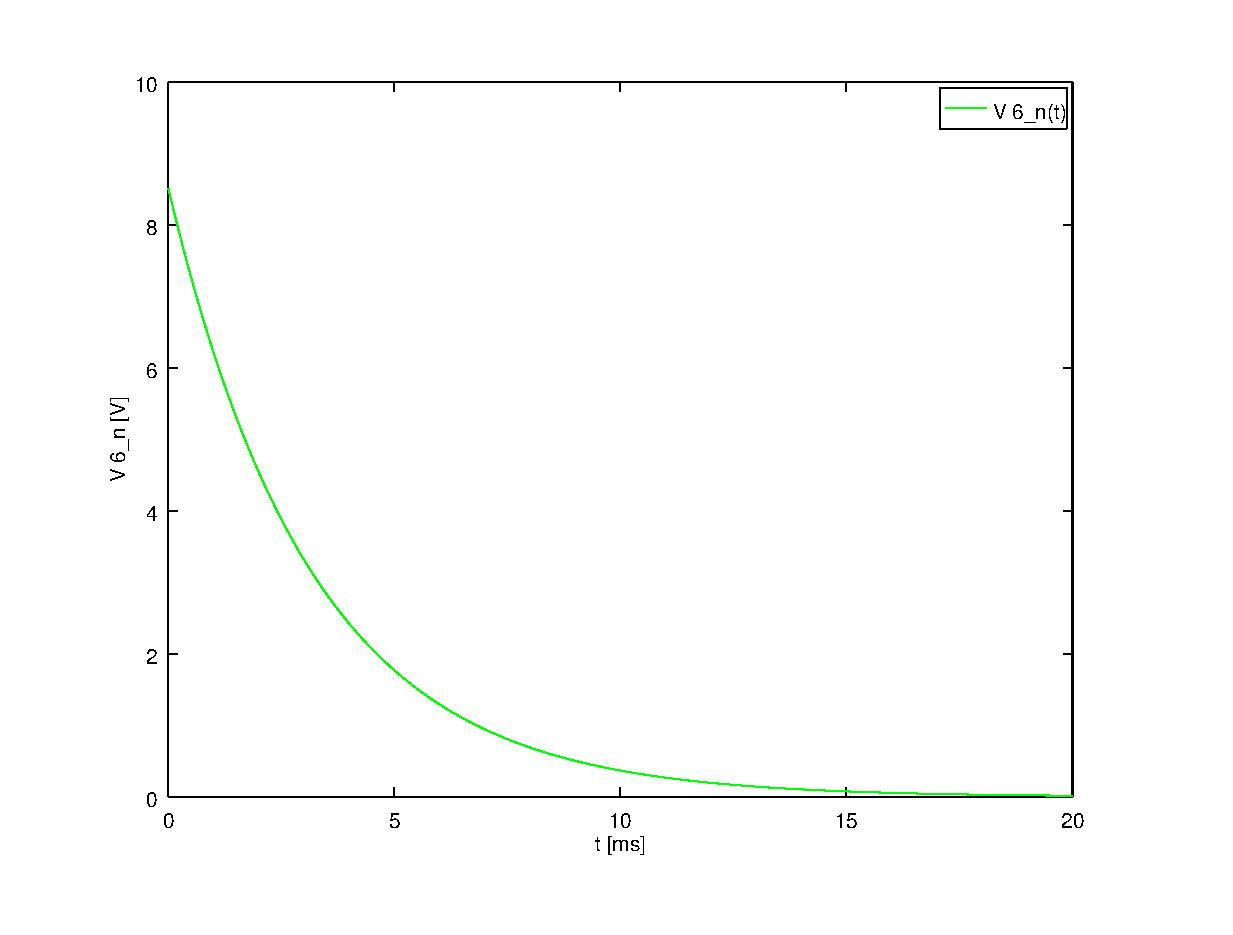
\includegraphics[width=0.6\linewidth]{natural.eps}
	\caption{Natural solution $V_{6n}$ in the interval $[0, 20]~ms$ plot.}
\label{fig:natural}
\end{figure}


\subsection{Forced Solution}

\paragraph{} In order to obtain the forced solution we must be able to solve the following equation.  

\begin{equation}
\begin{pmatrix}
1 & 0 & 0 & 0 & 0 & 0 & 0\\
-G1 & G1+G2+G3 & -G2 & -G3 & 0 & 0 & 0\\
0 & Kb+G2 & -G2 & -Kb & 0 & 0 & 0\\
-G1 & G1 & 0 & G4 & 0 & G6 & 0\\
0 & 0 & 0 & 0 & 0 & -G6-G7 & G7\\
0 & 0 & 0 & 1 & 0 & G6*Kd & -1\\
0 & -G3 & 0 & G3+G4+G5 & -G5-jwC & G6 & jwC\\
\end{pmatrix}
\begin{pmatrix}
V1\\
V2\\
V3\\
V5\\
V6\\
V7\\
V8\\
\end{pmatrix}
=
\begin{pmatrix}
-j\\
0\\
0\\
0\\
0\\
0\\
0\\
\end{pmatrix}
\end{equation}


The solution to this system is presented in the table below:


\begin{table}[h]
  \centering
  \begin{tabular}{|l|r|r|}
    \hline    
    {\bf Name} & {\bf Complex Amplitude [V]} & {\bf Phase [Degrees]}\\ \hline
    $V_{1}$ & 1.000000 & -90.000000\\ \hline
$V_{2}$ & 0.962760 & -90.000000\\ \hline
$V_{3}$ & 0.885131 & -90.000000\\ \hline
$V_{5}$ & 0.968250 & -90.000000\\ \hline
$V_{6}$ & 0.599056 & 98.067060\\ \hline
$V_{7}$ & 0.401350 & 90.000000\\ \hline
$V_{8}$ & 0.597330 & 90.000000\\ \hline 
  \end{tabular}
  \caption{Nodal analysis for phasor voltage in forced state.}
  \label{tab:phasor}
\end{table}


These values are needed to determine the forced solution $V_{6f}$, which is given by the following formula:

\begin{equation}
V_{6f}(t)=V_{6r}cos(\omega t+V_{6\phi});
\end{equation}

Where

\begin{equation}
\omega=2\pi f;
\end{equation}


\subsection{Final Total Solution}


The final total solution $V_6(t)$ is achieved by superimposing the natural and forced solutions. 



\begin{equation}
	V_6(t)=V_{6n}(t)+V_{6f}(t);
\end{equation}
By converting the phasors to real time functions for $f = 1 kHz$ and superimposing the natural and forced solutions, we can plot both $V_S(t)$ and $V_6(t)$ in the interval $[-5, 20]~ms$, as shown in the figure below:

\clearpage

\begin{figure}[h] \centering
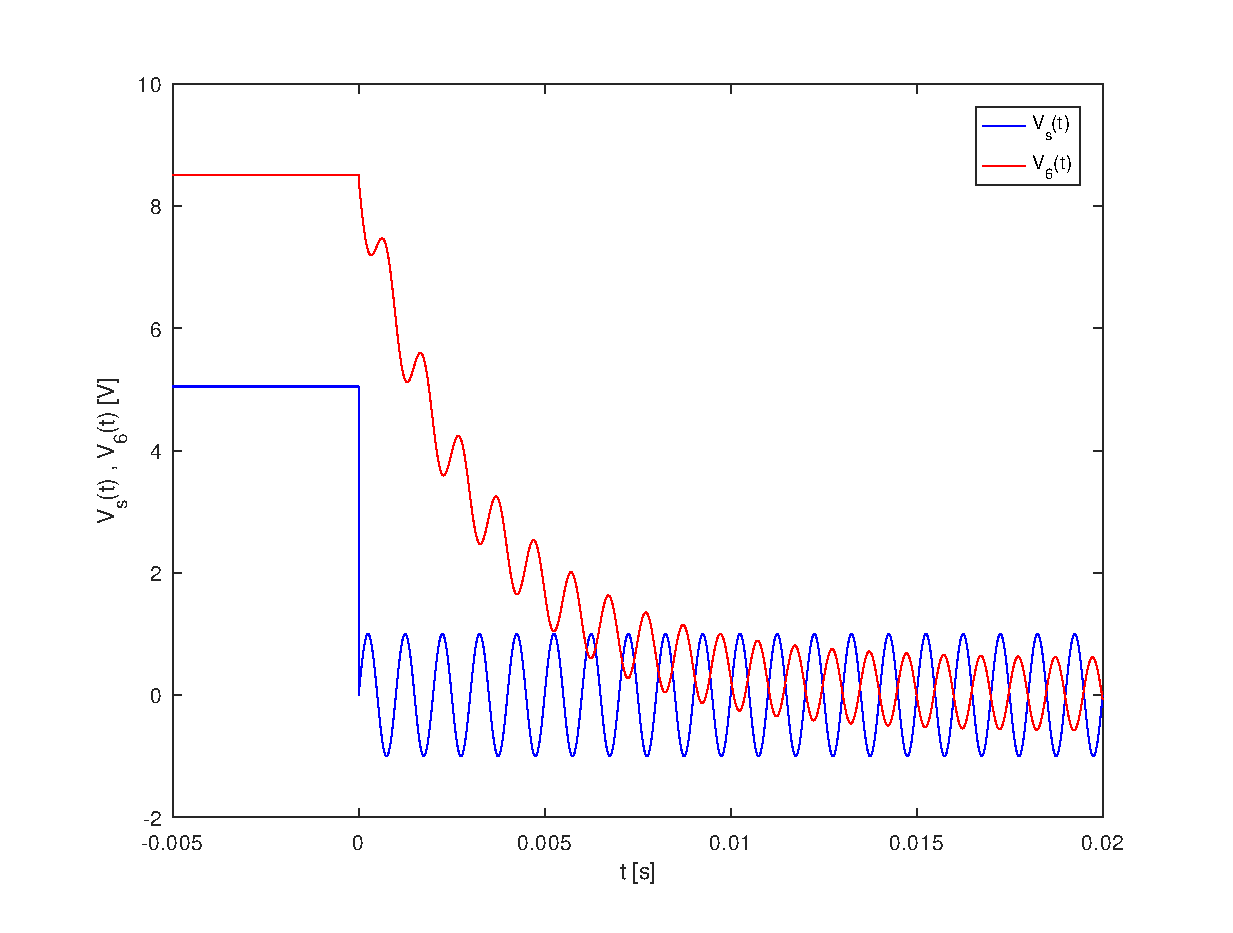
\includegraphics[width=0.7\linewidth]{total.eps}
\caption{Total solution of $V_{6}$ and $V_{s}$ plot.}
	\label{fig:total}
\end{figure}

As expected, both curves shown in Figure~\ref{fig:total} are constant for $t<0~s$. For $t>0~s$, we can see an evident negative exponencial behavior and an induced frequency in $V_{6}$.


\subsection{Frequency Responses}

Because $V_S(t) = sin(\omega t)$, the magnitude and phase are independent of the frequency $f$. This means that both the magnitude and phase are expected to be constant in the plots that follow.

The magnitude frequency response is given in Figure~\ref{fig:mag}.
The phase response for frequencies ranging from $0.1~Hz$ to $1~MHz$ is given in Figure~\ref{fig:phase}. The apparent discontinuity showed in the phase of $V(6)$ is in fact caused by the domain of the arctan function that is used to determined the phase, which is, in reality, continuous.

\clearpage

\begin{figure}[h] \centering
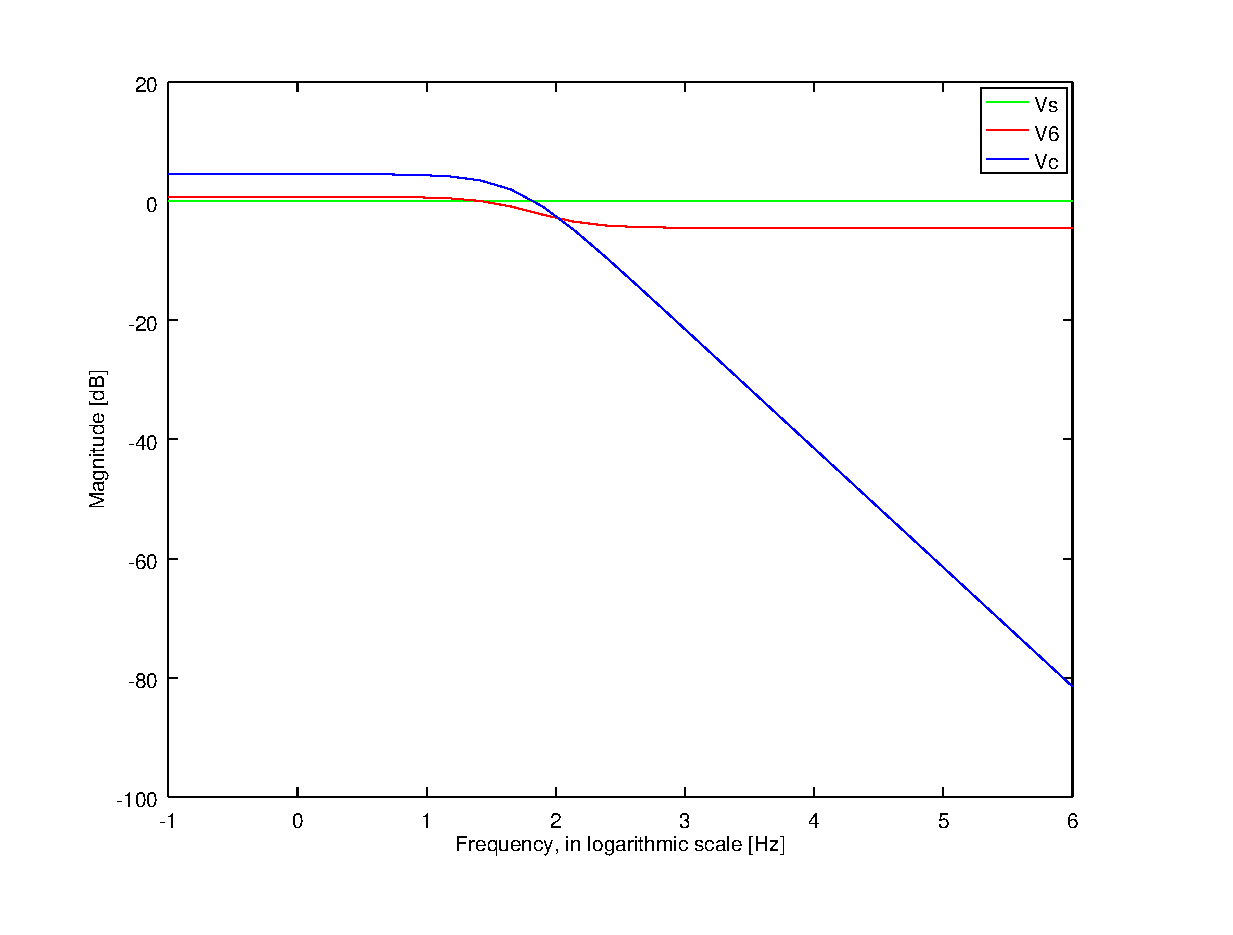
\includegraphics[width=0.5\linewidth]{magnitude.eps}
	\caption{Magnitude frequency response plot, in dB, of $V_{c}$, $V(6)$ and $V_{s}$.}
        \label{fig:mag}
\end{figure}


\begin{figure}[h] \centering
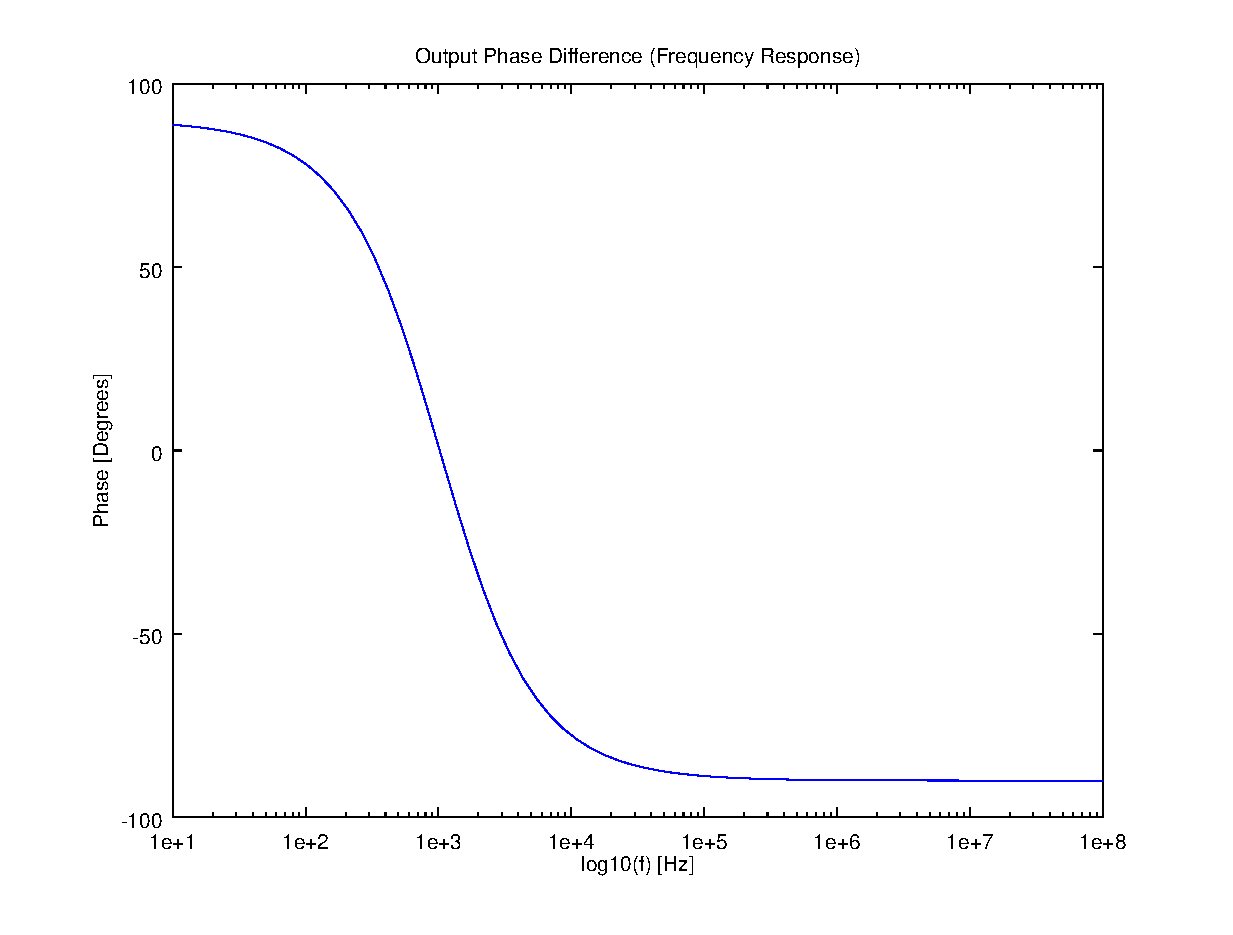
\includegraphics[width=0.7\linewidth]{phase.eps}
	\caption{Phase response plot, in degrees, of $V_{c}$, $V(6)$ and $V_{s}$.}
        \label{fig:phase}
\end{figure}
